\documentclass{article}
\usepackage{amsmath}
\usepackage{graphicx}
\usepackage{parskip}
\usepackage[a4paper, margin=6em]{geometry}
\usepackage{biblatex}

\addbibresource{sources.bib}

\title{Math meets Biology}
\author{Mario Kunz, Xaver Hanushevsky}
\date{March 2023}

\begin{document}

\maketitle

\newpage

\section{Positive Autoregulation}

System zweier Differentialgleichungen zum Beschreiben der positiven Autoregulation:

\begin{align*}
    \frac{d[\text{RNA}]}{dt}&=v_{max}\cdot\frac{[P]}{K+[P]}-k_{dr}\cdot[\text{RNA}] \\
    \frac{d[P]}{dt}&=k_s\cdot[\text{RNA}]-k_{dp}\cdot[P]
\end{align*}

\begin{tabular}{l l}
     $[\text{RNA}]$ & Konzentration der transkribierten mRNA \\
     $[P]$ & Konzentration des Proteins/Transkriptionsfaktor \\
     $v_{max}$ & maximale Geschwindigkeit der Transkription; entspricht $k_t\cdot [D_T]$ \\
     $k_t$ & Geschwindigkeitskonstante der Transkription \\
     $[D_T]$ & Konzentration der DNA bzw. TF-Bindungsstelle \\
     $K$ & Gleichgewichtskonstante der Bindung vom TF an die DNA-Bindungsstelle \\
     $k_{dr}$ & Geschwindigkeitskonstante der mRNA-Degradation \\
     $k_{dp}$ & Geschwindigkeitskonstante der Proteindegradation
\end{tabular}


\subsection{Numerische Lösung}

\subsubsection*{Gewählte Konstanten}
\begin{tabular}{l l}
    $\text{RNA}]_0$ & $0\text{ M}$ \\
    $[P]_0$ & $0.0005\text{ M}$ \\
    $v_{max}$ & $0.4\text{ M min$^{-1}$}$ \\
    $K_{diss}$ & $10^{-6}\text{ M}$ \\
    $k_{dp}$ & $0.056\text{ min$^{-1}$}$ \\
    $k_{dr}$ & $0.36\text{ min$^{-1}$}$ \\
    $k_s$ & $0.4\text{ min$^{-1}$}$
\end{tabular}

\begin{figure}[h]
    \centering
    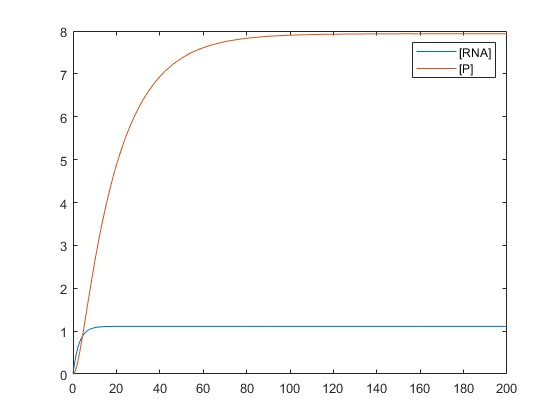
\includegraphics[width=0.8\linewidth]{images/positive_autoregulation.jpg}
\end{figure}

Konzentration von RNA und Protein nimmt so lange zu, bis der Steady-State erreicht wurde.\\
Würde das Experiment mit einer Proteinkonzentration über dem Steady-State-Wert starten, würde die Konzentration in der Folge auf diesen hinunterfallen.

\section{Negative Autoregulation}

System zweier Differentialgleichungen zum Beschreiben der negativen Autoregulation:

\begin{align*}
    \frac{d[\text{RNA}]}{dt}&=v_{max}\cdot\frac{K}{K+[P]}-k_{dr}\cdot[\text{RNA}] \\
    \frac{d[P]}{dt}&=k_s\cdot[\text{RNA}]-k_{dp}\cdot[P]
\end{align*}

\subsection{Numerische Lösung}

\subsubsection*{Gewählte Konstanten}
\begin{tabular}{l l}
    $[\text{RNA}]_0$ & $0\text{ M}$ \\
    $[P]_0$ & $0.0005\text{ M}$ \\
    $v_{max}$ & $0.4\text{ M min$^{-1}$}$ \\
    $K_{diss}$ & $10^{-6}\text{ M}$ \\
    $k_{dp}$ & $0.056\text{ min$^{-1}$}$ \\
    $k_{dr}$ & $0.36\text{ min$^{-1}$}$ \\
    $k_s$ & $0.4\text{ min$^{-1}$}$
\end{tabular}

\begin{figure}[h]
    \centering
    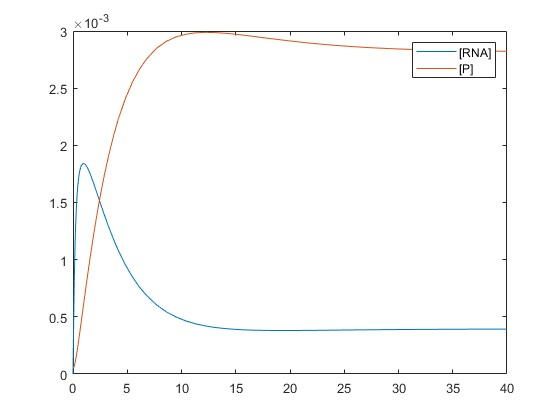
\includegraphics[width=0.8\linewidth]{images/negative_autoregulation.jpg}
\end{figure}

Konzentration von RNA und Protein überschiessen zuerst den Steady-State-Wert bevor sie darauf zurückfallen.

\newpage
\section{Draft Negative Autoregulation}
\subsection{Herleitung}
Wir wollen uns das Leben nicht zu schwer machen, deswegen nehmen wir uns ein einfaches Beispiel als Modell und wollen daran zeigen, wie wir ein mathematisches Modell anfertigen können.
Wir stellen uns das hypothetische Gen $A$ vor, dass für ein Protein $P$ codiert. Dieses Protein bindet jedoch auch als inhibitor and das Operon $O$ des Gens $A$ und verhindert die Transkription.\\
Uns interessiert die zeitliche Veränderung der Konzentration von $P$. //fix this
\begin{equation} \label{eq:1}
    \frac{d[\text{RNA}]}{dt}=[\text{RNA}]_{\text{Synthese}}-[\text{RNA}]_{\text{Abbau}}
\end{equation}
\subsubsection{Degradation der mRNA}
Da der Abbau einfacher zu verstehen ist, werden wir uns ihn als erstes anschauen. Wir werden um dieses ausgesprochen komplexe biologische System in ein vergleichbar sehr einfaches mathematisches Modell zu bringen viele Annahmen machen müssen. Für die Degradationsgeschwindigkeit nehmen wir einen konstanten Wert $k_{dr}$ an, den wir aus der Literatur\cite{lacoperon} nehmen. //rewrite// Die Rate müssen wir noch mit der Konzentration der mRNA multiplizieren, um die Anzahl der Zerfälle pro Zeit zu erhalten
\begin{equation} \label{eq:2}
    [\text{RNA}]_{\text{Abbau}}=[\text{RNA}] \cdot k_{dr}
\end{equation}
\subsubsection{RNA Synthese}
Die Synthese ist etwas komplexer, da wir hier die Konzentration von $P$ und die Affinität von $P$ and das Operon $O$ auch in betracht ziehen müssen. Auch hier nehmen wir wieder einen Wert aus der Literatur\cite{lacoperon} für die Affinität $K$. //...
\begin{equation} \label{eq:3}
    [\text{RNA}]_{\text{Synthese}}=v_{\text{max}} \cdot \frac{K}{K+[P]}
\end{equation}

\newpage
\section{Values scraped from places}
Lac-Operon\cite{lacoperon}
\begin{itemize}
    \item $A \cdot e^{-E/RT} = k$ = 853 L/mol*min at 37°C (?)
    \item transcription \& translation rate = 0.4 min$^{-1}$
    \item protein decay rate of U = 0.056 min$^{-1}$
    \item mRNA decay rate of V = 0.36 min$^{-1}$
\end{itemize}

\section*{Repressorfunktion des lac-Operons}

Eine wichtige Regulation des Lac-Operons ist die Repression des Gens, sofern eine geringe Lactose Konzentration in der Zelle vorherrscht. Dies wird erreicht, indem der Repressor \emph{LacI} nur an die DNA binden kann, wenn er nicht gleichzeitig mit Allolactose gebunden ist. Allolactose ist verwandt mit Lactose, welches die gleichen Zucker beinhaltet, diese aber anders verbunden sind. Das Enzym $\beta$-galactosidase (\emph{LacZ}) kann von der Zelle aufgenommene Lactose in Allolactose umwandeln. Die Produktion von Allolactose führt in der Folge zur weiteren Exprimierung des lac-operons und stellt somit eine positive Rückkopplung dar.
\par

\emph{Das Modell kann so noch nicht funktionieren}
\begin{itemize}
    \item Konzentration von Lactose geht noch ins negative, was sinnlos ist. Ist die vorliegende Kinetik überhaupt korrekt oder machen wir noch einen Überlegungsfehler?
    \item Erreicht die Konzentration von Lactose 0, sollte eigentlich gar nichts mehr produziert werde und ich würde eine abflachende Kurve erwarten. Aktuell bleiben die Konzentrationen von mRNA und Lactase auf einem Steady-State.
\end{itemize}

\begin{align*}
    \frac{d[\text{Lactose}]}{dt}&=-k_\text{lac}\cdot [\text{Lactase}] \\
    \frac{d[\text{Lactase}]}{dt}&=k_\text{translation}\cdot[\text{RNA}]-k_\text{ldeg}\cdot [\text{Lactase]}\\
    \frac{d[\text{RNA}]}{dt}&=k_\text{transcription}\cdot[\text{DNA}_\text{total}]\cdot\frac{K_\text{Diss DNA}}{K_\text{Diss DNA}+([\text{LacI}_\text{total}]\cdot\frac{[\text{Lactose}]}{K_\text{Diss LacI}+[\text{Lactose}]})}-k_\text{rdeg}\cdot[\text{RNA}]
\end{align*}

\printbibliography[title=References]

\end{document}
